\scanpage{76}
\uline{Lemme} 2 Se bornant aux anneaux
ess. de type fini sur un corps, on a
\[
\deleted{1^{\unsure{'+|\prime}}_n\Rightarrow 2'_{n+2}}.\qquad 1'_n+2'_{n+1}\Rightarrow2'_{n+2}
\]
[N.B. Et $2'_{n+2}\Rightarrow1'_{n+1}+2'_{n+2}$ grâce au lemme 1, OK]

En effet, on est sur un corps (sép clos $k$).
\deleted{et \unsure{le dernier|la dernière} de $f\in\unsure{\sqrt{0}} A$} \inserted{On peut supposer dans $2'_{n+2}$ que}
$f\in\unsure{\sqrt{0}|\not\sqrt{0}|\mathfrak m}A$ (sinon $X_f=\varnothing$ et tt est trivial]
\figure{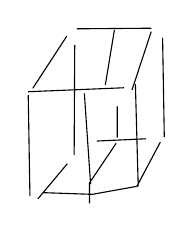
\begin{tikzpicture}[scale=.72]
\draw (0,.07)--(-.03,1.85) (.05,1.97)--(.65,2.89) (.83,3.02)--(2.14,3.03);
\draw (-.03,1.91)--(1.66,1.98) (1.33,2.03)--(1.49,3.00) (1.8,1.94)--(2.14,2.97);
\draw (2.34,2.86)--(2.37,1.11) (2.30,1.02)--(1.88,.23) (1.86,2.05)--(1.91,.24);
\draw (.14,.02)--(.66,.64) (.22,.13)--(1.10,.10)--(1.88,.24) (1.05,-.06)--(1.05,.30)--(1.52,1.00) (1.07,.28)--(.96,1.88);
\draw (.78,.79)--(.79,2.73) (1.18,1.04)--(2.05,1.08) (1.54,1.1)--(1.54,1.65);
\end{tikzpicture}}

\deleted{Alors $f$ \unsure{définit}} On peut supposer $A$
intègre si on y tient. Complétons
$f$ en un système de paramètres
\figure{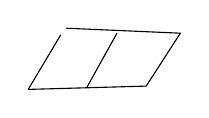
\begin{tikzpicture}[scale=.7]
\draw (.02,0)--(.61,.99) (.71,1.11)--(2.78,1.02)--(2.16,.06)--(.02,0);
\draw (1.08,.03)--(1.63,1.02);
\end{tikzpicture}}
$f_1=f,\unsure{f_1|f_2},\ldots f_{n+2}$, \deleted{les $n+1$ premiers}
\inserted{qui} définissent \deleted{$A_1=k\langle x_1,\ldots,x_n,\rangle\to A$}
$A'=k\langle x_1,\ldots x_{n+2}\rangle\to A$, Et $X$ \deleted{$=\operatorname{Spec}$}
est fini sur $X'=\operatorname{Spec} A'$, $U$ est l'image
inverse de $U'=X'_f$. On est
ramené à prouver que $\operatorname{cd}_{\ell}(U')\leq n$. Donc on
peut supposer $A=k\langle x_1,\ldots x_{n+2}\rangle$, \inserted{$f=x_1$.} Considérons
$B=k\langle x_1,\ldots x_{n+1}\rangle$ qui est de dim $n+1$, et
soit $Y=\operatorname{Spec} B$, $U=Y_f$. Considérons la projection
$V\longrightarrow U$. Par l'hyp. \deleted{de} $2'_{n+1}$, il suffira de
prouver que \deleted{\unsure{$f$}} $R^qf_*(F)$ est nul en
codim $i\unsure{\leq|<}q-1$, car alors $H^p(U,R^qf_*(F))\ne0$
$\Rightarrow\deleted{\unsure{pour}}\ p\leq n+1-(q-1)$. i.e. $p+q\leq n+2$,
d'où $H^i(V,F)\ne0\Rightarrow i\leq n+2$.

% slanted
\margin{Attention : \unsure{condition|conditions} \unsure{un|en} \unsure{moins} ?}
% archive sheet number: 75
